\documentclass[12pt]{article}
\newcommand{\ReportShortTitle}{Cá nhân -- Hồ Sĩ Phú}
\usepackage[a4paper,top=2.1cm,bottom=2.2cm,left=2.6cm,right=2.2cm,headheight=15pt]{geometry}
\usepackage{fontspec}
\setmainfont{Times New Roman}
\setsansfont{Arial}
\setmonofont{Menlo}[Scale=0.86]
\usepackage{microtype}
\usepackage{setspace}
\setstretch{1.22}
\usepackage{parskip}
\setlength{\parindent}{1.1cm}
\setlength{\parskip}{3pt}

\usepackage{xcolor}
% Hệ màu đơn sắc: chỉ dùng đen, trắng và các mức xám để in ấn chuyên nghiệp.
\definecolor{Primary}{gray}{0}
\definecolor{Secondary}{gray}{0}
\definecolor{Accent}{gray}{0.72}
\definecolor{SoftBlue}{gray}{0.94}
\definecolor{SoftGray}{gray}{0.97}
\definecolor{Success}{gray}{0}
\definecolor{Warning}{gray}{0}
% Màu chỉ dùng bên trong khối mã nguồn.
\definecolor{CodeKeyword}{HTML}{1F4E79}
\definecolor{CodeComment}{HTML}{3F6B45}
\definecolor{CodeString}{HTML}{8A4B08}

\usepackage{graphicx}
\usepackage{booktabs}
\usepackage{longtable}
\usepackage{tabularx}
\usepackage{array}
\usepackage{makecell}
\usepackage{multirow}
\usepackage{enumitem}
\usepackage{amsmath,amssymb}
\usepackage{tikz}
\usetikzlibrary{arrows.meta,positioning,shapes.geometric,fit}
\usepackage[most]{tcolorbox}
\usepackage{listings}
\usepackage{needspace}
\renewcommand{\lstlistingname}{Đoạn mã}
\renewcommand{\lstlistlistingname}{Danh sách đoạn mã}
\renewcommand{\contentsname}{MỤC LỤC}
\usepackage{titlesec}
\usepackage{fancyhdr}
\usepackage{lastpage}
\usepackage{hyperref}
\hypersetup{colorlinks=true,linkcolor=Primary,urlcolor=Secondary,citecolor=Primary,pdfborder={0 0 0}}

\setlist[itemize]{leftmargin=1.2cm,itemsep=2pt,topsep=3pt}
\setlist[enumerate]{leftmargin=1.2cm,itemsep=2pt,topsep=3pt}
\renewcommand{\arraystretch}{1.25}
\newcolumntype{Y}{>{\raggedright\arraybackslash}X}
\newcolumntype{C}[1]{>{\centering\arraybackslash}p{#1}}
\newcolumntype{L}[1]{>{\raggedright\arraybackslash}p{#1}}

\titleformat{\section}{\Large\bfseries\color{Primary}}{\thesection.}{0.55em}{}
\titleformat{\subsection}{\large\bfseries\color{Secondary}}{\thesubsection.}{0.5em}{}
\titleformat{\subsubsection}{\normalsize\bfseries\color{Primary}}{\thesubsubsection.}{0.5em}{}
\titlespacing*{\section}{0pt}{16pt}{7pt}
\titlespacing*{\subsection}{0pt}{11pt}{5pt}

\pagestyle{fancy}
\fancyhf{}
\fancyhead[L]{\small\color{Primary}\textbf{ĐỒ ÁN ESP32-S3}}
\fancyhead[R]{\small\color{Secondary}\ReportShortTitle}
\fancyfoot[L]{\small Nhóm 3 thành viên}
\fancyfoot[R]{\small Trang \thepage/\pageref{LastPage}}
\renewcommand{\headrulewidth}{0.5pt}
\renewcommand{\footrulewidth}{0.4pt}

\newtcolorbox{summarybox}[1][Tóm tắt]{
  enhanced, breakable, colback=SoftBlue, colframe=Secondary,
  title=\textbf{#1}, coltitle=white, colbacktitle=Secondary,
  boxrule=0.7pt, arc=2mm, left=3mm, right=3mm, top=2mm, bottom=2mm
}
\newtcolorbox{evidencebox}[1][Minh chứng]{
  enhanced, breakable, colback=SoftGray, colframe=Primary,
  title=\textbf{#1}, coltitle=white, colbacktitle=Primary,
  boxrule=0.6pt, arc=1.5mm, left=3mm, right=3mm, top=2mm, bottom=2mm
}
\newtcolorbox{warningbox}[1][Lưu ý]{
  enhanced, breakable, colback=Accent!12, colframe=Warning,
  title=\textbf{#1}, coltitle=white, colbacktitle=Warning,
  boxrule=0.6pt, arc=1.5mm, left=3mm, right=3mm, top=2mm, bottom=2mm
}

\lstdefinestyle{firmware}{
  language=C++,
  basicstyle=\ttfamily\fontsize{8.35}{10.2}\selectfont,
  keywordstyle=\color{CodeKeyword}\bfseries,
  commentstyle=\color{CodeComment}\itshape,
  stringstyle=\color{CodeString},
  numbers=left,
  numberstyle=\sffamily\fontsize{6.8}{8.2}\selectfont\color{black!48},
  numbersep=9pt,
  frame=lines,
  framerule=0.45pt,
  rulecolor=\color{black!68},
  backgroundcolor=\color{white},
  framesep=5.5pt,
  breaklines=true,
  breakatwhitespace=false,
  breakindent=1.25em,
  columns=fullflexible,
  keepspaces=true,
  showstringspaces=false,
  tabsize=2,
  escapeinside={(*@}{@*)},
  xleftmargin=1.1em,
  xrightmargin=0.25em,
  framexleftmargin=1.0em,
  framexrightmargin=0.45em,
  aboveskip=9pt,
  belowskip=10pt,
  abovecaptionskip=6pt,
  belowcaptionskip=0pt,
  captionpos=b
}

% Chú thích tiếng Việt được render bằng XeLaTeX ngay trong khung mã.
\newcommand{\VNCodeComment}[1]{%
  \parbox[t]{0.93\linewidth}{%
    \raggedright\color{CodeComment}\sffamily\fontsize{7.7}{9.1}\selectfont\itshape
    \textcolor{CodeComment}{\textbf{//}}\enspace #1}%
}

\newcommand{\ProjectTitle}{THIẾT BỊ ĐEO THEO DÕI SỨC KHỎE, PHÁT HIỆN TÉ NGÃ VÀ ĐỊNH VỊ DÙNG ESP32-S3}
\newcommand{\GroupMembers}{Phạm Hùng Tiến -- Hồ Sĩ Phú -- Quách Gia Thịnh}
\newcommand{\ReportDate}{Tháng 8 năm 2026}
\newcommand{\RepositoryURL}{https://github.com/PhamHungTien/esp32-s3-health-monitor}
\newcommand{\RepositoryDisplay}{github.com/PhamHungTien/esp32-s3-health-monitor}
\newcommand{\UniversityName}{TRƯỜNG ĐẠI HỌC KHOA HỌC TỰ NHIÊN}
\newcommand{\UniversitySystem}{ĐẠI HỌC QUỐC GIA THÀNH PHỐ HỒ CHÍ MINH}
\newcommand{\FacultyName}{KHOA ĐIỆN TỬ -- VIỄN THÔNG}

\newcommand{\CoverInstitution}{%
  \centering
  
\includegraphics[height=2.8cm]{assets/branding/hcmus_logo_user.png}\par
  \vspace{0.2cm}
  {\sffamily\bfseries\small\color{Primary}\UniversitySystem\par}
  \vspace{2pt}
  {\sffamily\bfseries\fontsize{16}{20}\selectfont\color{Primary}\UniversityName\par}
  \vspace{3pt}
  {\sffamily\bfseries\large\color{Secondary}\FacultyName\par}
  \vspace{0.35cm}
  {\color{Primary}\rule{0.84\textwidth}{1.0pt}\par}
}

\newcommand{\CoverBands}{%
  \begin{tikzpicture}[remember picture,overlay]
    \fill[Primary] (current page.north west) rectangle ([yshift=-4.5mm]current page.north east);
    \fill[Secondary] (current page.south west) rectangle ([yshift=3mm]current page.south east);
  \end{tikzpicture}%
}

\newcommand{\CoverField}[2]{%
  \noindent
  \begin{minipage}[t]{0.35\linewidth}
    \raggedright\strut\sffamily\bfseries\color{Primary}#1
  \end{minipage}\hfill
  \begin{minipage}[t]{0.61\linewidth}
    \raggedright\strut\sffamily\color{black}#2
  \end{minipage}\par
}

\hypersetup{
  pdftitle={\ProjectTitle\space -- \ReportShortTitle},
  pdfauthor={\GroupMembers},
  pdfsubject={Báo cáo đồ án thiết bị theo dõi sức khỏe dùng ESP32-S3},
  pdfkeywords={ESP32-S3, MAX30102, OLED, IMU, GPS, nhịp tim, SpO2, té ngã}
}

\newcommand{\MakeReportCover}[4]{%
  \hypersetup{pageanchor=false}
  \begin{titlepage}
    \thispagestyle{empty}
    \centering
    \CoverBands
    \vspace*{0.05cm}
    \CoverInstitution
    \vspace{0.45cm}
    {\sffamily\bfseries\normalsize\color{Secondary} BÁO CÁO ĐỒ ÁN\par}
    \vspace{0.35cm}
    {\sffamily\bfseries\fontsize{18}{23}\selectfont\color{Primary}\ProjectTitle\par}
    \vspace{0.6cm}
    \begin{tcolorbox}[width=0.84\textwidth,colback=SoftBlue,colframe=Secondary,arc=1.8mm,boxrule=0.8pt,left=4mm,right=4mm,top=2.7mm,bottom=2.7mm]
      \centering{\sffamily\bfseries\normalsize\color{Secondary} #1\par}
    \end{tcolorbox}
    \vfill
    \begin{tcolorbox}[width=0.84\textwidth,colback=white,colframe=Primary!48,arc=1.2mm,boxrule=0.6pt,left=6mm,right=6mm,top=4.5mm,bottom=4.5mm]
      \raggedright
      \CoverField{Người thực hiện}{#2}
      \vspace{2.1mm}
      \CoverField{Mã số sinh viên}{#3}
      \vspace{2.1mm}
      \CoverField{Nhóm}{03 thành viên}
      \vspace{2.1mm}
      \CoverField{Phạm vi báo cáo}{#4}
    \end{tcolorbox}
    \vfill
    {\sffamily\footnotesize\color{Secondary}\GroupMembers\par}
    \vspace{0.2cm}
    {\sffamily\footnotesize\color{Primary}\textbf{Mã nguồn đồ án: }
      \href{\RepositoryURL}{\RepositoryDisplay}\par}
    \vspace{0.2cm}
    {\sffamily\bfseries\small\color{Primary}Thành phố Hồ Chí Minh, \ReportDate\par}
    \vspace{0.2cm}
  \end{titlepage}
  \hypersetup{pageanchor=true}
  \clearpage
}

\newcommand{\MakeGroupCover}[1]{%
  \hypersetup{pageanchor=false}
    \begin{titlepage}
    \thispagestyle{empty}
    \centering
    \CoverBands
    \vspace*{0.05cm}
    \CoverInstitution
    \vspace{0.45cm}
    {\sffamily\bfseries\normalsize\color{Secondary} BÁO CÁO ĐỒ ÁN\par}
    \vspace{0.35cm}
    {\sffamily\bfseries\fontsize{18}{23}\selectfont\color{Primary}\ProjectTitle\par}
    \vspace{0.6cm}
    \begin{tcolorbox}[width=0.84\textwidth,colback=SoftBlue,colframe=Secondary,arc=1.8mm,boxrule=0.8pt,left=4mm,right=4mm,top=2.7mm,bottom=2.7mm]
      \centering{\sffamily\bfseries\normalsize\color{Secondary} #1\par}
    \end{tcolorbox}
    \vfill
    \begin{tcolorbox}[width=0.84\textwidth,colback=white,colframe=Primary!48,arc=1.2mm,boxrule=0.6pt,left=6mm,right=6mm,top=4.5mm,bottom=4.5mm]
      \sffamily
      {\bfseries\color{Primary}THÀNH VIÊN THỰC HIỆN\par}
      \vspace{3mm}
      \begin{tabularx}{\linewidth}{C{1.1cm} Y C{3.0cm}}
        \toprule
        \textbf{STT} & \textbf{Họ và tên} & \textbf{MSSV}\\
        \midrule
        1 & Phạm Hùng Tiến & 24207043\\
        2 & Hồ Sĩ Phú & 24207101\\
        3 & Quách Gia Thịnh & 24207105\\
        \bottomrule
      \end{tabularx}
    \end{tcolorbox}
    \vfill
    {\sffamily\footnotesize\color{Primary}\textbf{Mã nguồn đồ án: }
      \href{\RepositoryURL}{\RepositoryDisplay}\par}
    \vspace{0.2cm}
    {\sffamily\bfseries\small\color{Primary}Thành phố Hồ Chí Minh, \ReportDate\par}
    \vspace{0.2cm}
  \end{titlepage}
  \hypersetup{pageanchor=true}
  \clearpage
}

\newcommand{\Code}[1]{\texttt{#1}}
\newcommand{\OK}{\textcolor{Success}{\textbf{Đạt}}}
\newcommand{\Implemented}{\textcolor{Secondary}{\textbf{Đã cài đặt}}}
\newcommand{\NeedTest}{\textcolor{Warning}{\textbf{Cần thử thêm}}}
\newcommand{\Pending}{\textcolor{Warning}{\textbf{Cần hiệu chuẩn}}}


\begin{document}
\MakeReportCover{BÁO CÁO CÔNG VIỆC CÁ NHÂN}{Hồ Sĩ Phú}{24207101}{Đo nhịp tim và ước lượng SpO$_2$ bằng MAX30102}

\begin{summarybox}[Nội dung phụ trách]
Trong đồ án, em phụ trách cảm biến MAX30102: cấu hình thanh ghi, đọc FIFO, xử lý tín hiệu RED/IR, phát hiện ngón tay, tính nhịp tim và ước lượng SpO$_2$.
\end{summarybox}

\section{Mục tiêu công việc}

Phần xử lý cần chuyển dữ liệu RED/IR thành BPM và SpO$_2$, đồng thời nhận biết trường hợp chưa đặt ngón tay hoặc tín hiệu chưa ổn định. Giá trị chỉ được hiển thị khi thỏa các điều kiện về biên độ và khoảng nhịp.

\section{Công việc đã thực hiện}

\subsection{Cấu hình và thu FIFO}

Em cấu hình MAX30102 bằng các thanh ghi điều khiển: reset, con trỏ FIFO, chế độ SpO$_2$, độ phân giải ADC, tốc độ lấy mẫu 100 mẫu/giây và dòng LED. Mỗi phần tử FIFO gồm ba byte RED và ba byte IR, được ghép thành số 18 bit. Số mẫu chờ được xác định từ hai con trỏ ghi/đọc để tránh mất dữ liệu.

\begin{figure}[htbp]
  \centering
  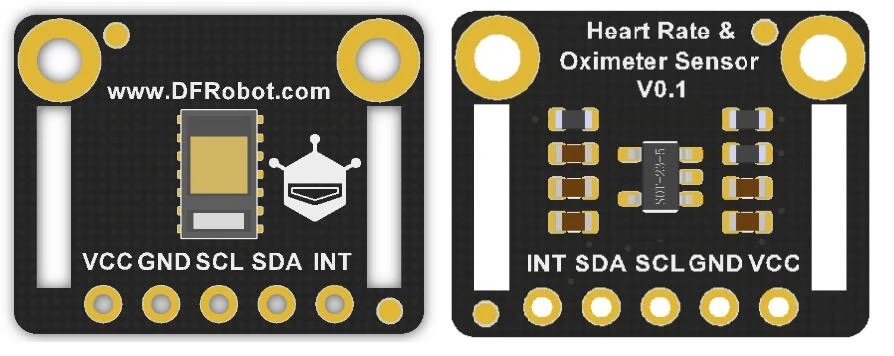
\includegraphics[width=0.72\textwidth,height=5.0cm,keepaspectratio]{assets/components/max30102_board_overview.jpg}
  \caption{Mô-đun tham chiếu dùng MAX30102 với các chân VCC, GND, SCL, SDA và INT. Bo thực tế của nhóm được xác nhận bằng địa chỉ I2C 0x57; hình dạng PCB có thể khác. Nguồn ảnh: \href{https://wiki.dfrobot.com/sen0344/docs/19237}{DFRobot}.}
  \label{fig:phu-max30102}
\end{figure}

\begin{center}
\small
\begin{tabularx}{0.94\textwidth}{C{2.0cm} C{2.0cm} Y}
\toprule
\textbf{Thanh ghi} & \textbf{Giá trị} & \textbf{Chức năng trong chương trình}\\
\midrule
0x09 & 0x40/0x03 & Reset, sau đó chạy chế độ RED--IR\\
0x04--0x06 & 0x00 & Xóa con trỏ ghi, tràn và đọc FIFO\\
0x08 & 0x1F & Cho phép FIFO quay vòng, không lấy trung bình trong chip\\
0x0A & 0x27 & Thang ADC 4.096 nA, 100 mẫu/giây, xung 411 $\mu$s\\
0x0C/0x0D & 0x24 & Dòng LED đỏ và hồng ngoại khoảng 7,2 mA\\
\bottomrule
\end{tabularx}
\normalsize
\end{center}

Mỗi mẫu được gắn thời điểm tăng 10 ms. Thời gian mẫu do đó không phụ thuộc vào thời gian vẽ OLED hay in Serial, giúp khoảng RR được tính nhất quán.

\subsection{Phát hiện ngón tay và tiền xử lý}

Giá trị IR nền khi không đặt tay đo được khoảng 330--400, trong khi đặt tay đạt khoảng 132.000--137.000. Em dùng hai ngưỡng nhận/nhả để trạng thái ngón tay không thay đổi liên tục. Khi rời tay, bộ đếm nhịp, cửa sổ AC/DC và các giá trị đo được xóa.

Thành phần DC được ước lượng bằng bộ lọc IIR chậm. Thành phần AC là hiệu giữa mẫu và DC; nó tiếp tục được làm mượt để giảm nhiễu cao tần. Tín hiệu sử dụng số thực đơn và không cần thư viện xử lý tín hiệu bên ngoài.

\Needspace{0.38\textheight}
\begin{lstlisting}[style=firmware,caption={Ngưỡng trễ nhận ngón tay và xóa trạng thái khi rời tay}]
bool hasFinger = ppg.fingerPresent ?
                   (irValue > 7000) : (irValue > 10000);
if (!hasFinger) {
  if (ppg.fingerPresent) PPG_ResetMetrics();
  state.dcRed = redValue;
  state.dcIr = irValue;
  return;
}

if (!ppg.fingerPresent) {
  ppg.fingerPresent = true;
  state.fingerStartMs = sampleTimeMs;
  state.dcRed = redValue;
  state.dcIr = irValue;
}
\end{lstlisting}

\begin{codeexplanation}
\CodeExplainLine{1}{Chọn ngưỡng IR theo trạng thái trước đó để tạo vùng trễ khi nhận hoặc bỏ ngón tay.}
\CodeExplainLine{2}{Khi đã nhận ngón tay dùng ngưỡng 7.000; khi chưa nhận dùng ngưỡng 10.000 để chống dao động.}
\CodeExplainLine{3}{Đi vào nhánh xử lý khi mẫu hiện tại không còn đủ điều kiện có ngón tay.}
\CodeExplainLine{4}{Nếu vừa chuyển từ có sang không có ngón tay thì xóa các kết quả đo của phiên trước.}
\CodeExplainLine{5}{Đặt mức nền kênh đỏ bằng mẫu hiện tại để bộ lọc khởi động lại đúng mức tín hiệu.}
\CodeExplainLine{6}{Đặt mức nền kênh hồng ngoại theo cùng nguyên tắc.}
\CodeExplainLine{7}{Dừng xử lý mẫu vì không được phép tính BPM hoặc SpO$_2$ khi chưa có ngón tay.}
\CodeExplainLine{8}{Kết thúc nhánh không có ngón tay.}
\CodeExplainLine{9}{Dòng trống tách phần loại bỏ mẫu với phần khởi tạo một phiên đo mới.}
\CodeExplainLine{10}{Kiểm tra đây có phải mẫu hợp lệ đầu tiên sau khi đặt ngón tay hay không.}
\CodeExplainLine{11}{Ghi nhận cảm biến đang có ngón tay.}
\CodeExplainLine{12}{Lưu thời điểm bắt đầu phiên đo để các bước sau biết tuổi của tín hiệu.}
\CodeExplainLine{13}{Khởi tạo mức nền kênh đỏ bằng mẫu đầu tiên của phiên đo.}
\CodeExplainLine{14}{Khởi tạo mức nền kênh hồng ngoại bằng mẫu đầu tiên của phiên đo.}
\CodeExplainLine{15}{Kết thúc khối khởi tạo phiên đo.}
\end{codeexplanation}

\subsection{Thuật toán nhịp tim}

Với cảm biến đặt ở đầu ngón, tín hiệu IR sau lọc dao động quanh đường nền. Trong 0,8 giây đầu, bộ lọc bám nhanh theo mức DC để loại xung lớn khi vừa đặt tay. Sau đó, đáy cục bộ vượt ngưỡng thích nghi được dùng làm mốc nhịp; khoảng trơ ngăn một nhịp bị đếm hai lần. Khoảng giữa hai nhịp hợp lệ $\Delta t$ được đổi sang BPM:

\[
  \mathrm{BPM}=\frac{60\,000}{\Delta t_{\mathrm{ms}}}.
\]

Chỉ các giá trị trong miền sinh lý được đưa vào bộ làm mượt. Chương trình bỏ 0,8 giây đầu để đường nền ổn định; khoảng RR hợp lệ đầu tiên sau đó được hiển thị ngay. Các nhịp kế tiếp chỉ được dùng nếu không lệch quá 22 BPM so với giá trị đang có. Trong điều kiện đặt tay tốt, kết quả thường xuất hiện sau khoảng 2--3 giây.

\subsection{\texorpdfstring{Ước lượng SpO$_2$}{Ước lượng SpO2}}

Trong mỗi cửa sổ, em tính thành phần DC và độ mạnh AC của hai kênh. Tỷ số chuẩn hóa được xác định bởi:

\[
 R=\frac{AC_{RED}/DC_{RED}}{AC_{IR}/DC_{IR}},
 \qquad SpO_2\approx a-bR.
\]

Kết quả được chặn trong miền hợp lệ, làm mượt giữa các cửa sổ và chỉ công nhận khi biên độ AC đủ lớn, DC khác 0 và tỷ số nằm trong vùng hợp lý. Chỉ số chất lượng $Q$ được giữ trong nhật ký Serial để hỗ trợ kiểm tra; màn hình người dùng không hiện nhãn TỐT/VỪA/YẾU.

\Needspace{0.22\textheight}
\begin{warningbox}[Giới hạn đo SpO$_2$]
Giá trị SpO$_2$ hiện là ước lượng phục vụ đồ án, chưa phải thiết bị y tế. Các lần thử gần nhất cho kết quả khoảng 90--96\%; cần thu cặp dữ liệu với máy đo chuẩn, khớp lại hệ số $a,b$ và kiểm tra trên nhiều người trước khi kết luận độ chính xác.
\end{warningbox}

\Needspace{0.48\textheight}
\section{Các đoạn mã quyết định}

\subsection{Xác nhận nhịp và khởi tạo BPM}

Bộ dò sử dụng đáy cục bộ, ngưỡng theo biên độ tín hiệu và khoảng trơ 450 ms. Khoảng RR hợp lệ đầu tiên được xuất ngay; các nhịp sau chỉ được nhận nếu không lệch quá 22 BPM so với giá trị đang có.

\Needspace{0.42\textheight}
\begin{lstlisting}[style=firmware,caption={Điều kiện phát hiện nhịp và hiển thị BPM sớm}]
float slope = state.filtered - state.previousFiltered;
float peakThreshold = state.envelope * 0.95f;
if (peakThreshold < 100.0f) peakThreshold = 100.0f;

if (state.previousSlope < 0.0f && slope >= 0.0f &&
    state.previousFiltered < -peakThreshold &&
    now - ppg.lastBeatMs > 450) {
  if (ppg.lastBeatMs != 0) {
    uint32_t interval = now - ppg.lastBeatMs;
    if (interval >= 480 && interval <= 1500) {
      float instantBPM = 60000.0f / interval;
      if (!ppg.heartRateValid) {
        ppg.bpm = instantBPM;
        ppg.heartRateValid = true;
      } else if (fabsf(instantBPM - ppg.bpm) <= 22.0f) {
        ppg.bpm = 0.80f * ppg.bpm + 0.20f * instantBPM;
      }
    }
  }
  ppg.lastBeatMs = now;
}
\end{lstlisting}

\begin{codeexplanation}
\CodeExplainLine{1}{Tính độ dốc của tín hiệu đã lọc so với mẫu ngay trước đó.}
\CodeExplainLine{2}{Đặt ngưỡng đỉnh bằng 95\% biên độ bao hiện tại để ngưỡng tự thích nghi với cường độ tín hiệu.}
\CodeExplainLine{3}{Giới hạn ngưỡng tối thiểu ở 100 để nhiễu nhỏ không bị nhận nhầm thành nhịp.}
\CodeExplainLine{4}{Dòng trống phân tách bước chuẩn bị ngưỡng với bước xác nhận đỉnh.}
\CodeExplainLine{5}{Phát hiện thời điểm độ dốc đổi từ âm sang không âm, tức một cực tiểu của dạng sóng đã đảo.}
\CodeExplainLine{6}{Yêu cầu biên độ cực tiểu vượt ngưỡng thích nghi vừa tính.}
\CodeExplainLine{7}{Buộc hai nhịp cách nhau hơn 450 ms để loại bỏ đỉnh giả quá gần.}
\CodeExplainLine{8}{Chỉ tính khoảng RR khi hệ thống đã lưu được thời điểm của một nhịp trước.}
\CodeExplainLine{9}{Tính khoảng thời gian giữa hai nhịp liên tiếp theo mili giây.}
\CodeExplainLine{10}{Chỉ chấp nhận khoảng RR từ 480 đến 1.500 ms, tương ứng vùng nhịp hợp lý của nguyên mẫu.}
\CodeExplainLine{11}{Đổi khoảng RR sang nhịp mỗi phút bằng công thức 60.000 chia cho số mili giây.}
\CodeExplainLine{12}{Kiểm tra đây có phải giá trị BPM hợp lệ đầu tiên của phiên đo hay không.}
\CodeExplainLine{13}{Hiển thị trực tiếp BPM tức thời ở nhịp hợp lệ đầu tiên.}
\CodeExplainLine{14}{Đánh dấu BPM đã sẵn sàng để giao diện không tiếp tục hiện dấu chờ.}
\CodeExplainLine{15}{Với các nhịp sau, chỉ nhận giá trị mới nếu chênh lệch không quá 22 BPM.}
\CodeExplainLine{16}{Làm mượt bằng 80\% giá trị cũ và 20\% giá trị mới để giảm rung số.}
\CodeExplainLine{17}{Kết thúc nhánh cập nhật BPM sau khi đã có kết quả trước đó.}
\CodeExplainLine{18}{Kết thúc khối kiểm tra khoảng RR hợp lệ.}
\CodeExplainLine{19}{Kết thúc khối yêu cầu phải có nhịp trước.}
\CodeExplainLine{20}{Lưu thời điểm đỉnh hiện tại; đỉnh này sẽ làm mốc cho lần tính RR tiếp theo.}
\CodeExplainLine{21}{Kết thúc điều kiện xác nhận đỉnh nhịp.}
\end{codeexplanation}

Đây là nhánh quyết định trực tiếp khi nào BPM được phép xuất hiện trên màn hình và cách giá trị tiếp tục được làm mượt.

\Needspace{0.40\textheight}
\subsection{\texorpdfstring{Ratio-of-ratios cho SpO$_2$}{Ratio-of-ratios cho SpO2}}
\begin{lstlisting}[style=firmware,caption={Tính tỷ số quang và giá trị SpO2 nguyên mẫu}]
float redRms = sqrtf((float)(state.redSquareSum /
                             state.windowSamples));
float irRms = sqrtf((float)(state.irSquareSum /
                            state.windowSamples));
float ratio = (redRms / state.dcRed) / (irRms / state.dcIr);

if (ratio > 0.2f && ratio < 2.0f) {
  float estimatedSpO2 = constrain(110.0f - 25.0f * ratio,
                                  70.0f, 100.0f);
  ppg.spo2 = ppg.spo2Valid ?
             0.8f * ppg.spo2 + 0.2f * estimatedSpO2 : estimatedSpO2;
}
\end{lstlisting}

\begin{codeexplanation}
\CodeExplainLine{1}{Tính giá trị hiệu dụng của thành phần AC kênh đỏ từ tổng bình phương trong cửa sổ.}
\CodeExplainLine{2}{Chia tổng bình phương cho số mẫu trước khi lấy căn để nhận RMS đúng chuẩn.}
\CodeExplainLine{3}{Bắt đầu phép tính RMS tương tự cho kênh hồng ngoại.}
\CodeExplainLine{4}{Hoàn tất phép tính RMS kênh hồng ngoại theo số mẫu của cửa sổ.}
\CodeExplainLine{5}{Tính tỷ số chuẩn hóa giữa AC/DC của kênh đỏ và AC/DC của kênh hồng ngoại.}
\CodeExplainLine{6}{Dòng trống tách phép tính tỷ số với bước kiểm tra miền hợp lệ.}
\CodeExplainLine{7}{Chỉ ước lượng SpO$_2$ khi tỷ số nằm trong miền 0,2 đến 2,0 để loại mẫu bất thường.}
\CodeExplainLine{8}{Áp dụng đường hiệu chuẩn tuyến tính của nguyên mẫu để đổi tỷ số quang sang phần trăm SpO$_2$.}
\CodeExplainLine{9}{Giới hạn kết quả trong khoảng 70--100\% để tránh giá trị hiển thị phi thực tế.}
\CodeExplainLine{10}{Kiểm tra hệ thống đã có kết quả SpO$_2$ hợp lệ từ cửa sổ trước hay chưa.}
\CodeExplainLine{11}{Nếu đã có thì làm mượt 80/20; nếu chưa có thì dùng ngay ước lượng đầu tiên.}
\CodeExplainLine{12}{Kết thúc nhánh cập nhật SpO$_2$.}
\end{codeexplanation}

Hai hệ số 110 và 25 là đường cong nguyên mẫu. Báo cáo không xem chúng là hệ số y tế đã hiệu chuẩn.

\section{Nhật ký khối lượng}

\begin{tabularx}{\textwidth}{L{7.6cm} C{2.1cm} Y}
\toprule
\textbf{Hạng mục} & \textbf{Thời lượng} & \textbf{Đầu ra}\\
\midrule
Cấu hình thanh ghi và FIFO 100 Hz & 5 giờ & Luồng RED/IR liên tục\\
Phát hiện ngón tay và reset trạng thái & 4 giờ & Không xuất số khi rời tay\\
Lọc DC/AC và ngưỡng thích nghi & 5 giờ & Tín hiệu xung ổn định\\
Phát hiện nhịp, khoảng trơ, BPM & 7 giờ & BPM quan sát 72--83\\
Ratio-of-ratios và làm mượt SpO$_2$ & 6 giờ & Giá trị cùng cờ hợp lệ\\
Đánh giá chất lượng, thử nghiệm & 3 giờ & $Q$, bảng kết quả và giới hạn\\
\midrule
\textbf{Tổng} & \textbf{30 giờ} & \textbf{Đã cài đặt; SpO$_2$ cần hiệu chuẩn}\\
\bottomrule
\end{tabularx}

\section{Kết quả kiểm thử}

\begin{tabularx}{\textwidth}{L{4.4cm} L{4.2cm} Y}
\toprule
\textbf{Tình huống} & \textbf{Quan sát} & \textbf{Kết luận}\\
\midrule
Không đặt ngón tay & IR khoảng 330--400; BPM/SpO$_2$ ở WAIT & \OK\\
Đặt ngón tay ổn định & IR khoảng 132.000--137.000 & Nhận diện biên độ rõ\\
Sau thời gian hội tụ & BPM khoảng 72--83 qua các lần thử & \OK\\
Ước lượng SpO$_2$ thử nghiệm & Khoảng 90--96\% trong các lần thử gần nhất & \Pending\\
Rút ngón tay & Xóa cờ hợp lệ và cửa sổ đo & \OK\\
\bottomrule
\end{tabularx}

\section{Kết quả đạt được}

\begin{evidencebox}[Các giá trị đầu ra]
Phần chương trình MAX30102 gồm các hàm khởi tạo, đọc FIFO, xử lý từng mẫu, phát hiện ngón tay, tính BPM, tính ratio-of-ratios và đánh giá chất lượng tín hiệu. Các giá trị dùng chung gồm \Code{fingerPresent}, \Code{bpm}, \Code{spo2}, \Code{signalQuality}, \Code{heartRateValid} và \Code{spo2Valid}.
\end{evidencebox}

\section{Nhận xét và hướng hoàn thiện}

Thuật toán đã phát hiện được ngón tay và cho BPM ổn định trong điều kiện người đo giữ yên. SpO$_2$ hiện mới là giá trị ước lượng. Cần thu thêm dữ liệu đối chứng để hiệu chỉnh hệ số và đánh giá ảnh hưởng của lực ép, chuyển động và ánh sáng ngoài.

\end{document}
